\section{Independent Variables}

This section presents the chosen independent variables from our 21 self trackers. The dataset spans a wide variety of different variables. For instance, some people track their dependent variables such as sleep quality and productivity and how these are affected by the amount of time spent doing physical activities such as swimming, running and weightlifting. We categorize all these relevant activities into \enquote{exercise}. Similarly, other people track their dependent variables such as weight and productivity by measuring the intake of a certain drink such as coffee or tea. We also categorize these independent variables into \enquote{beverage intake}. By contrast, some independent variables were unique to some participants in which case we discuss them together in one subsection. By categorizing the different independent variables in this manner, this paper focuses on five main categories which range from Exercise, beverage intake, use of electronic devices, weather conditions, and miscellaneous. This section first demonstrates a chart in the Fig.\ref{fig:chart} followed by the detailed descriptions of each category. 

\begin{figure}[!t]\centering
%\begin{wrapfigure}{o}{\textwidth}\centering
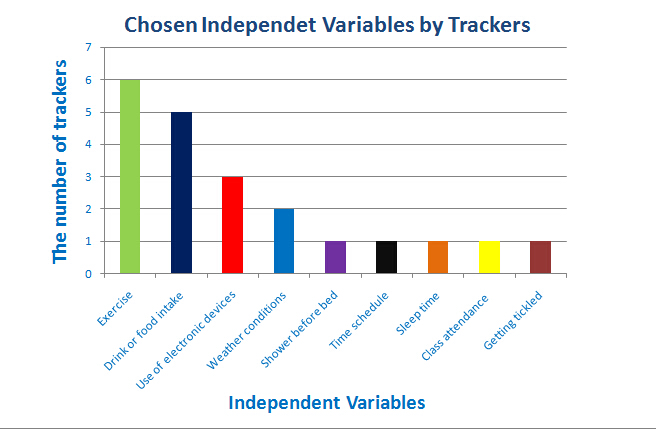
\includegraphics[width=1.0\columnwidth]{images/independent_variables.jpg}
\caption{\footnotesize Independent Variables studied by the participants \label{fig:chart} 
}%\end{wrapfigure}
\end{figure}

\subsection{Exercise}
Most people are insecure about their body shape. Some would like to build up muscles while others may want to lose or maintain weight. Nowadays, exercise has become one of the most popular activities in people's lives. Users often used exercise as an independent variable. It was evaluated in terms of its effects on different dependent variables, including but not limited to all three of the most common dependent variables discussed in this paper. There were reported variations in duration, occurrence, scheduling, and types of exercise as part of experiments\textquotesingle  designs. Exercise is a general term which includes a variety of activities. Of our 21 self trackers, three chose running, one chose swimming, one focused on steps walked per day, and finally one weight lifted as their independent variable. Therefore, \enquote{exercise} is one of the most common independent variables being chosen in six out of our 21-participant repository reports.
 
\subsection{Beverage Intake}
A new study presented at the American Academy of Neurology\textquotesingle s 67th Annual Meeting in Washington, DC, suggests yet another potential health benefit of coffee consumption: it could reduce the risk of multiple sclerosis. People are curious about the effects of different beverages on personal health and behavior. Four self trackers chose beverage intake as their independent variables to test out their dependent variables ranging from mood, productivity, pH level, well being, sleep quality and weight gain/loss. The drinks that our trackers used include coffee, green tea, cider apple vinegar water and beer. In this paper, we looked at the relationship between a certain type of drink consumption/intake and overall mortality or productivity.
 
\subsection{Use of electronic devices}
In the 21st century people are spending more and more time on their electronic devices;Tasks can be easily accomplished using computers and social media connection on apps like Facebook and Twitter are becoming increasingly popular. However, basking in the blue glow of iPads, smartphones and other electronic devices before bedtime could be disrupting sleep patterns more profoundly than we realize, and even affecting our long-term health, according to a new study published Monday in the Proceedings of the National Academy of Sciences. One of our trackers chose the use of electronic devices after 9PM as an independent variable to test out sleep quality and the effect on dreams. And another tracker chose the usage of computer during the day to see how the time spent on the computer affects sleep quality. Similarly, one tracker wants to see how productivity is affected by using cell phone over a certain amount of time.
 
\subsection{Weather conditions}
As most of the nation suffers through some of the hottest or coldest temperatures on record in summer or winter, people are asking the question of how exactly weather impact our mood? For instance, how does hot weather affect our mood? Does it make us more aggressive or even more violent? Does rain make us sad? Do cold temperatures make us feel more like wanting to hunker down, hibernate, and isolate ourselves from others? So in our 28-day experiment, one of our trackers choose mean of daily temperature as independent variable to identify laziness and the total millimeters of hot beverage intake. Another tracker uses weather conditions (daily temperature, the amount of precipitation and wind speed) to find out how these conditions affect the exercise (exercise types, exercise occurrence and duration of exercise).
\subsection{Miscellaneous}
Considering the fact that some independent variable is used only by one tracker, these independent variables are not common ones that people use to determine their hypotheses. One tracker is interested in seeing how sleep quality and heart rate are affected by taking a shower before bed. One tracker uses time schedule to test out mood, sleep quality and productivity. One tracker also tries to find out what is the perfect time to go to bed in order to produce the best sleep quality. Additionally, there are two interesting cases where one tracker evaluates mood, sleep quality and weight loss by getting tickled with a hypothesis that getting tickled has positive effect on all those dependent variables and where one tracker identifies how productivity and money spent online are affected by class attendance. 

This paper mainly focuses on the first four categories in that those independent variables are utilized by most of our trackers. Additionally, this statistics seems more likely to be able to be applied to the broader general population as well. This paper does not try to include as many as independent variables but to narrow down to concrete ones and see how dependent variables are affected by these popular independent variables. 
